\documentclass[letterpaper, 10 pt, conference]{ieeeconf}
\overrideIEEEmargins

% The following packages can be found on http:\\www.ctan.org
\usepackage{graphics} % for pdf, bitmapped graphics files
\usepackage{epsfig} % for postscript graphics files
%\usepackage{mathptmx} % assumes new font selection scheme installed
\usepackage{times} % assumes new font selection scheme installed
%\usepackage{lmodern}
\usepackage{amsmath} % assumes amsmath package installed
\usepackage{amssymb} % assumes amsmath package installed
\usepackage[activate={true, nocompatibility}, final, tracking=true, kerning=true, spacing=true, factor=1000, stretch=20, shrink=20]{microtype} % nicer typesetting

\usepackage{fixmath}
\usepackage{array}
\usepackage{multirow}
\usepackage{bm}
\usepackage{mathrsfs}
\newcolumntype{C}{>{$}c<{$}}
\newcolumntype{R}{>{$}r<{$}}

\usepackage{lmodern}

%\newcommand{\matr}[1]{\bm{#1}}
%%\newcommand{\matr}[1]{#1}
\newcommand{\matr}[1]{\mathbold{#1}}
\newcommand{\graph}[1]{\mathcal{#1}}

\newcommand{\T}{\mathrm{T}}
\newcommand{\upto}{\mathinner {\ldotp \ldotp}}

\DeclareMathOperator*{\argmin}{arg\min}

\title{\LARGE \bf Portfolio Optimization Using Preference Flow Based on Statistical Arbitrage}
\author{Lovre Mr\v{c}ela et al.}

\begin{document}

  \maketitle
  \thispagestyle{empty}
  \pagestyle{empty}
    
  \begin{abstract}
    
  A new algorithm for portfolio optimization is proposed which is based on statistical arbitrage, with potential method used to obtain the most preferred assets.
  A graph that represents preference flow among financial assets (i.e., if an edge exists going from asset $\mathbold{A}$ to asset $\mathbold{B}$, then $\mathbold{A}$ is preferred over $\mathbold{B}$) is constructed at each time step, using the modified version of statistical arbitrage.
  Then, the preference of each asset is calculated, using the potential method\cite{caklovic}, from which the most preferred assets are selected into the portfolio for each time step.
  
  Method has been tested on dataset (TODO: which dataset), by simulating the portfolio obtained by the algorithm, including the trading cost of 0.1\%.
  Sharpe ratios over 1.0 were observed.
  
  \end{abstract}
  
  \section{INTRODUCTION}
  
  The task of portfolio optimization is to try to enhance various criteria, which most of the time include maximization of expected return and minimization of deviation\dots
  
  Classical statistical arbitrage methods take into account some pair of assets whose prices behave similarly during certain period of time measured by cointegration, correlation, or some other measure of similarity; then try to find a moment in time when those assets' prices go out of what was statistically considered as `normal' range.
  When such opportunities show up, we can take advantage of them by predicting, with a certain statistical confidence, that they will return to the `normal' range once again in the next time step, and do the trading accordingly to this prediction.
  
  In this paper, we present a new method that uses predictions obtained by statistical arbitrage method, with confidence as a proxy for describing the preference relations between pairs of assets.
  Next, a graph is formed based on those relations, so that in-depth analysis of assets' interaction with each other might be performed.
  Finally, assets are put into order by preference, and picked into the portfolio.
  The idea of this method is to create a generalization of statistical arbitrage methods that will be more robust and perform better when working on a larger number of assets.
  
%  Each asset is compared to all other assets while looking for such specific deviations, so, in general, this algorithm performs better where there is larger number of assets.
  
  
%  Approach taken in this paper relies on statistical anomalies which are detected by observing past windows of time at each time step.
%  In this paper, approach was to create a portfolio using a large number of assets among which exist pairs that behave similarly during certain period.
%  At each time step, a past window of time is observed for finding pairs that abruptly stop behaving similarly.
  
  \section{CONCEPTS AND METHODS}
  
  Following are descriptions of the key components in the algorithm: graph of preference flow, and choosing assets for the portfolio...
  
  \subsection{Preference relations and utility function}
  
  Let $\Omega$ be any set of entities.
  Preference relation $\succ_{\Omega \times \Omega}$ is a \textit{strict weak ordering} that describes the way humans prefer some entity over another.
  This relation is specific in that it is ($\forall x, y, z \in \Omega$):
  \begin{itemize}
    \item \textit{irreflexive}: every entity $x$ is not preferrable over itself, %($\neg \left( x \succ x \right)$),
    \item \textit{asymmetrical}: if $x$ is preferrable over some $y$, then $y$ is not preferrable over $x$, %($x \succ y \Rightarrow \neg \left( y \succ x \right)$),
    \item \textit{transitive}: if $x$ is preferrable over $y$, and $y$ is preferrable over $z$, then $x$ is also preferrable over $z$, %($x \succ y \wedge y \succ z \Rightarrow x \succ z$),
    \item \textit{transitive in incomparability} (noting that $x$ and $y$ may be \textit{incomparable}, i.e. neither $x$ is preferrable over $y$, nor $y$ is preferrable over $x$): if $x$ is incomparable with $y$, and $y$ is incomparable with $z$, then $x$ is also incomparable with $z$.
  \end{itemize}

  We naturally assume this kind of relation when describing relationships among the assets.
  Determining that some asset is preferred over another is an easier task than assigning a preference rank to each asset individually, especially when the number of assets becomes large.
  However, the latter is more useful for decision making, and therefore it is desirable to find a way of sorting assets in the order of preference.
  
  Utility function $U\colon \Omega \to \mathbb{R}$ is mapping from entities to real numbers, in such way that order of the mapping corresponds to the preference order of the entities, i.e. $\forall x, y \in \Omega, U(x) > U(y) \Rightarrow x \succ y$.
  One such mapping is obtained by using potential method that is described later in this paper.
  In addition to ordering of the entities, utility function also provides a magnitude of preference for particular entity, and hence it is more informative when it comes to the decision making.
  
  \subsection{Graph of preference flow}
  
  Graph of preference flow is a simple weighted directed graph whose nodes represent entities, edges represent preference for one entity over another, and edge weights correspond to the strength of the preferences.
  In case of missing edge between two nodes, it is considered that neither entity is preferable over another (incomparability).
  The graph as a whole describes preference flow among the entities.
  An example of graph is shown on Fig. \ref{fig:graph}.
  
  \begin{figure}[h]
    \centering
    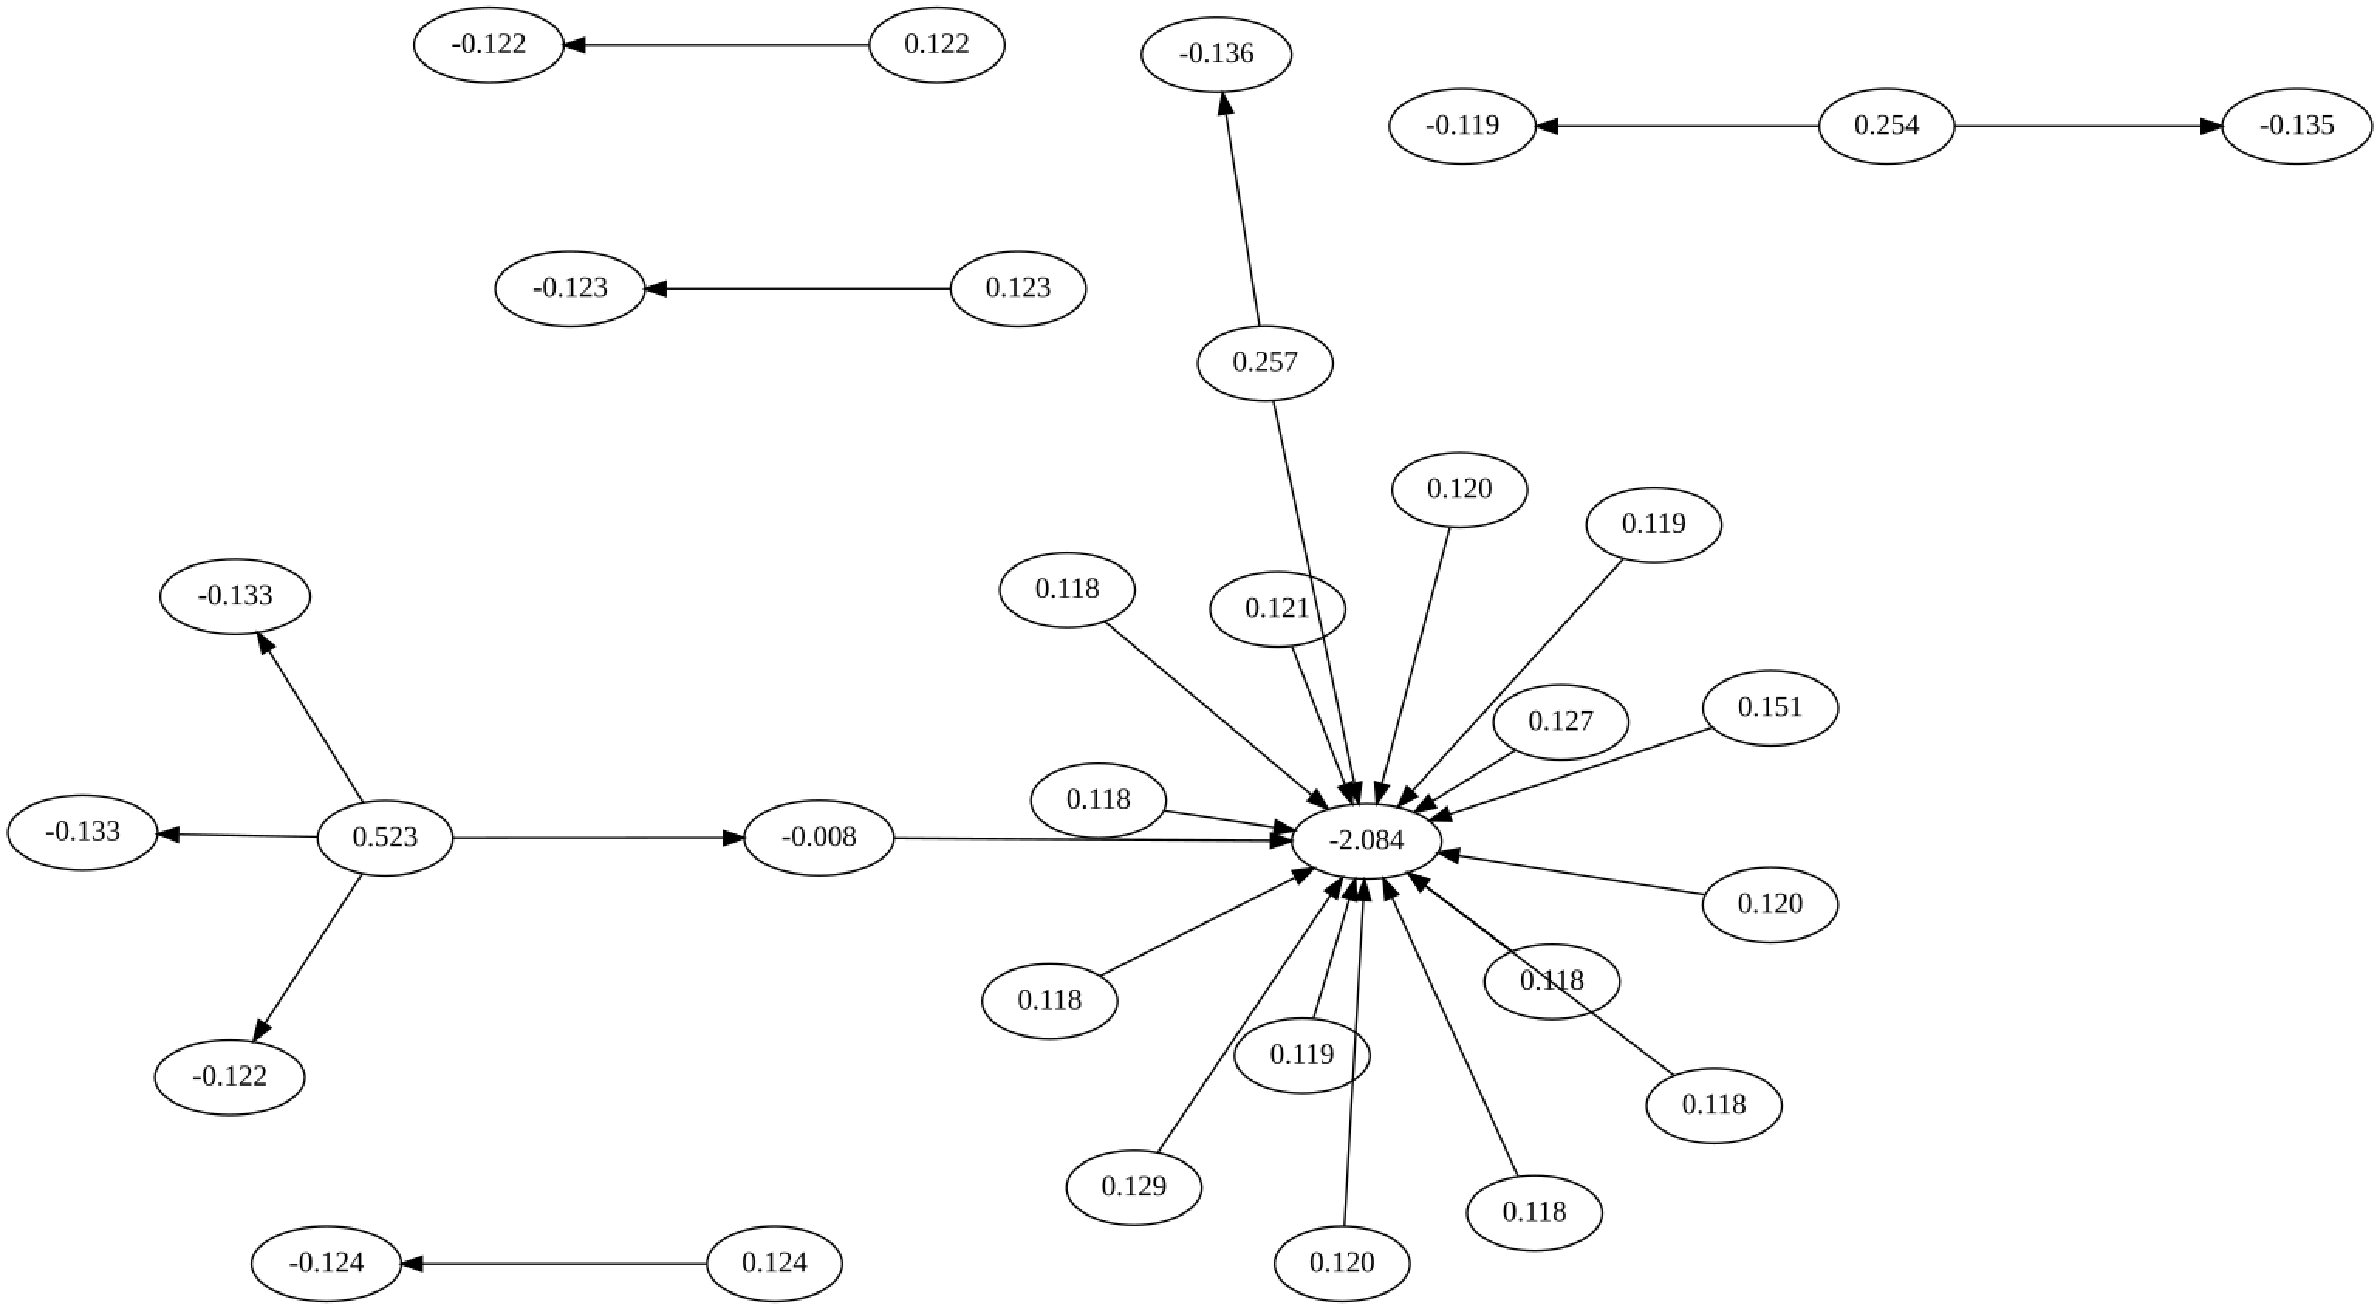
\includegraphics[width=\columnwidth]{graphics/graph.pdf}
    \caption{(TODO: put image with weights on edges) An example of a graph of preference flow. Asset number and calculated preference are inscribed in each node, and preference flows are shown on edges.}
    \label{fig:graph}
  \end{figure}
  
  Connections in this graph impose a preference relation among entities that are in the graph, in a way that an edge that goes from node $A$ to node $B$ means that $A$ is preferred over $B$.
  It is the case that neither node is in relation with itself (irrelexivity), and that no multiple connections are allowed between two nodes (implies asymmetry).
  However, problems arise with the aforementioned properties of transitivity, and transitivity in incomparability, which may not hold for an arbitrary instance of the graph.
  This imposed preference relation should preferably be consistent, but when it comes to larger number of entities, it may become infeasible to construct a graph with such qualities.
  Instead of aiming at consistency of relations, we devise a consistency measure and use it as an additional parameter in decision making.
  
  The measure of this preference flow is determined by a statistical arbitrage method, and it corresponds to the magnitude of a pair of assets prices ratio going out of what is considered statistically confident range.
  This is illustrated on Fig. \ref{fig:devmag}.
  
  \begin{figure}[h]
    \centering
    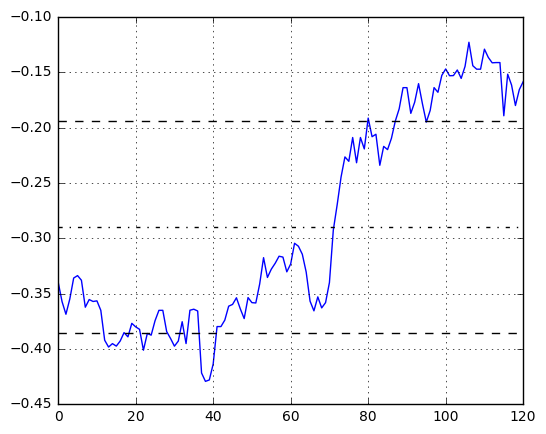
\includegraphics[width=0.9\columnwidth]{graphics/deviation-magnitude.png}
    \caption{(TODO: put a better image, this is just for a placeholder) Log price difference of a pair of assets during period of $T + 1$ time steps.
    During the last observed timestep, it goes (TODO: broj) times standard deviations away from mean value of past time window of size $T$.
    This would be measure of preference flow from asset with higher price to the asset with lower price.}
    \label{fig:devmag}
  \end{figure}

  The main idea of preference flow is that preference of a particular node depends on amount of preference flowing in and out of it.
  This allows for some kind of generalized statistical arbitrage over multiple assets at a time.
   
  \subsection{Potential method}
  \label{sub:potential}
  From previously obtained graph it is possible to tell which pair of assets has the highest preference flow.
  However, it is not yet possible to directly tell which are the most or least preferrable assets, or obtain the measure of preference for individual assets.
  To calculate preferences for each node in the graph, we use the potential method\cite{caklovic}.
  The potential of a node corresponds to difference in amount of flow going in and out of the node.
  
  A concise summary of the method is as follows:
  \begin{enumerate}
    \item For the observed graph $\graph{G}$, let there be a total of $N$ nodes, and maximum of $E = \binom{N}{2}$ edges, in case of a complete graph.
    
    \item If $\graph{G}$ is not complete, we complete it by adding edges to it with weight 0 (direction doesn't matter).
    Thus, from now on $\graph{G}$ is a complete graph with $\binom{N}{2}$ edges.
    % In our case, graphs will be incomplete for most of the time, but they may be \textsl{supplemented} (TODO: opposite of `reduced') to complete graphs, if we treat missing edges as edges of weight 0 (direction doesn't matter).
    
    \item Let $\matr{B}$ be the $E \times N$ incidence matrix of $\graph{G}$.
%    $\matr{B}$ has following properties:
%    \begin{enumerate}
%      \item each row corresponds to an edge in the graph, and each column to a node,
%      \item for every edge in the graph going from node $i$ to node $j$, there is a corresponding row that has $-1$ and $1$ in columns that correspond to nodes $i$ and $j$ respectively,
%      \item the remainder of elements in the matrix are zeros.
%    \end{enumerate}

    \item Let $\matr{f}$ be $E \times 1$ vector that contains edge weights (i.e. preference flows).
    Order of the edges must be the same as order of the edges in $\matr{B}$.
    As mentioned before, in place of missing edges we simply put 0.
    
    \item Let $\matr{\phi}$ be $N \times 1$ vector that contains potentials of each node, in order that is the same as order of the nodes in $\matr{B}$.
    
    \item Now, if $\graph{G}$ was consistent, then $\matr{B}$, $\matr{\phi}$, and $\matr{f}$ would satisfy the equation
    \begin{equation}
    \label{eq:flowformula}
    \matr{B} \matr{\phi} = \matr{f}.
    \end{equation}
    Equation (\ref{eq:flowformula}) simply means that the difference between potential of any two nodes should result result in weight of the edge between them.
    This is possible only for consistent graphs, and most of the time our graphs will be inconsistent.
    In that case we try to find an approximate solution $\matr{\phi^*}$ that minimizes the square error:
    \begin{gather}
    \matr{\phi^*} = \argmin_{\matr{\phi}} \left\{ \left \lVert \matr{B} \matr{\phi} - \matr{f}\textsl{} \right \rVert ^ 2 \right\} \nonumber \\ 
    \Downarrow \nonumber \\
    \label{eq:derivative}
    \frac{\partial \left \lVert \matr{B} \matr{\phi^*} - \matr{f} \right \rVert ^ 2}{\partial \matr{\phi^*}} = \mathbf{0}.
    \end{gather}
    Solving (\ref{eq:derivative}) via commonly used techniques of matrix calculus brings us to the following equation:
    \begin{equation}
    \label{eq:flow}
    \matr{B}^\T \matr{B} \matr{\phi^*} = \matr{B}^\T \matr{f}.
    \end{equation}
    Equation (\ref{eq:flow}) determines $\matr{\phi^*}$ up to a constant (i.e. solution has one degree of freedom), so the following constraint is also included:
    \begin{equation}
    \label{eq:sumiszero}
    \matr{j}^\T \matr{\phi^*} = 0
    \end{equation}
    where $\matr{j}$ is vector of ones with same dimension as $\matr{\phi^*}$.
    This ensures an unique solution for which total amounts of positive and negative potential will be equal.
    
    \item Joining the previous two equations together by adding (\ref{eq:sumiszero}) to each row in (\ref{eq:flow}) results in:
    \begin{align}
    \matr{B}^\T \matr{B} \matr{\phi^*} + \matr{J} \matr{\phi^*} &= \matr{B}^\T \matr{f} \nonumber \\
    \label{eq:joined}
    \left[\matr{B}^\T \matr{B} + \matr{J} \right] \matr{\phi^*} &= \matr{B}^\T \matr{f},
    \end{align}
    where $\matr{J}$ is a matrix of ones with same dimension as $\matr{B}^\T \matr{B}$.
    Finally, solving (\ref{eq:joined}) for $\matr{\phi^*}$ gives us:
    \begin{equation}
    \label{eq:final}
    \matr{\phi^*} = \left[\matr{B}^\T \matr{B} + \matr{J} \right]^{-1} \matr{B}^\T \matr{f}.
    \end{equation}
    \item Furthermore, the term $\left[ \matr{B}^\T \matr{B} + \matr{J} \right]^{-1}$ in (\ref{eq:final}) can be simplified to $\frac{1}{N} \matr{I}$ due to $\matr{B}^\T \matr{B}$ being the Laplace matrix of a complete graph; thus, we can simplify (\ref{eq:final}) some more:
    \begin{equation}
    \matr{\phi^*} = \frac{1}{N} \matr{B}^\T \matr{f},
    \end{equation}
    to get as computationally optimal expression as possible.
    
    \item Afterwards, we can calculate the reconstruction $\matr{f}^*$ of preference  flow by simply plugging back $\matr{\phi^*}$ into (\ref{eq:flowformula}):
    \begin{equation}
    \matr{f^*} = \matr{B} \matr{\phi^*}.
    \end{equation}
    The reconstructed preference flow $\matr{f^*}$ compared to the original preference flow $\matr{f}$ may even contain some new and/or lose some old edges.
    In addition, $\matr{B}$, $\matr{\phi^*}$, and $\matr{f^*}$ now describe a consistent graph $\graph{G}^*$.
    This allows now to define a consistency measure $\kappa$ as follows:
    \begin{equation}
    \label{eq:consistency}
    \kappa = \frac{\left \lVert \matr{f^*} \right \rVert}{\left \lVert \matr{f} \right \rVert}.
    \end{equation}
    Equation (\ref{eq:consistency}) represents the cosine of the angle between $\matr{f}$ and $\matr{f^*}$ in the column space of matrix $\matr{B}$.
    Consistency measure $\kappa$ tells us how consistent graph $\graph{G}$ was, compared to the $\graph{G}^*$.
    $\kappa$ ranges from 0 to 1, with 0 being full inconsistency (virtually unreachable), and 1 meaning full consistency.
    
  \end{enumerate}
  
  \section{ALGORITHM} 
  
  Parameters of the algorithm are:
  \begin{itemize}
    \item $T$ - length of the past time window,
    \item $\alpha$ - the deviation threshold,
    \item $\beta$ - asset selection threshold.
  \end{itemize}
  
  Let there be total of $N$ assets in $D$ days.
  Let price of asset $i$ at the time step $t$ be $a_i^{(t)}$, for $i \in {\left[1 \upto N\right]}$ and $t \in {\left[0 \upto D-1\right]}$.
  The log prices $b_i^{(t)}$, and log price differences $c_{i,j}^{(t)}$ between assets $i$ and $j$ are obtained as follows:
  \begin{equation} b_i^{(t)} = \log\left(a_i^{(t)}\right) \end{equation}
  \begin{equation} c_{i,j}^{(t)} = b_i^{(t)} - b_j^{(t)}, \end{equation}
  and rolling means $m_{i,j}^{(t)}$ and standard deviations $d_{i,j}^{(t)}$ of log price differences over the past time window of size $T$ are obtained as follows:
   
  \begin{equation}
    \label{eq:mean}
    m_{i,j}^{(t)} = \frac{1}{T}\sum_{\tau = t - T}^{t - 1} c_{i,j}^{(\tau)}
  \end{equation}
  \begin{equation}
    \label{eq:deviation}
    d_{i,j}^{(t)} = \sqrt{\frac{1}{T}\sum_{\tau=t - T}^{t - 1} \left(c_{i,j}^{(\tau)} - m_{i,j}^{(t)} \right)^2}.
  \end{equation}
  
  Note that in summation used in (\ref{eq:mean}, \ref{eq:deviation}) time step $t$ was intentionally excluded, therefore summation goes only to $t - 1$.
  We use these calculations as basis for creating the portfolio.
  
%  Note that period over which means and standard deviations of log price differences are calculated does not include time step $t$.
%  Also note that calculating them separately for each time step $t$ is rather computationally inefficient when dealing with rolling windows of data.
%  Therefore, it is advisable to use a rolling algorithm as described in the appendix.
%  On that note, $c_{i,j}^{(t)}$, $m_{i,j}^{(t)}$, and $d_{i,j}^{(t)}$ may be more efficiently stored if stored contiguously in memory as a matrix, using following coding scheme: a pair $(i, j)$, where $i < j$, should be encoded to $k$ as:
%  \begin{equation} k = N \cdot (i - 1) + j - 1 - \left. i \cdot (i + 1) \middle/ 2\right., \end{equation}
%  and decoded from $k$ as:
%  \begin{equation} i = \left\lfloor N + 1/2 - \sqrt{(N + 1/2)^2 - 2(N + k)} \right\rfloor, \end{equation}
%  \begin{equation} j = k + i \cdot \left.(i + 1) \middle/ 2\right. - N \cdot (i - 1) + 1. \end{equation}
%  An example of proposed coding is shown on figure \ref{fig:coding}.
%  
%  \begin{figure}[h]
%    \centering
%    \begin{tabular}{C|CCCCC}
%      i/j & 1 & 2 & 3 & 4 & 5 \\ \hline
%      1 & \cdot & 0 & 1 & 2 & 3 \\
%      2 & \cdot & \cdot & 4 & 5 & 6 \\
%      3 & \cdot & \cdot & \cdot & 7 & 8 \\
%      4 & \cdot & \cdot & \cdot & \cdot & 9 \\
%      5 & \cdot & \cdot & \cdot & \cdot & \cdot
%    \end{tabular}
%    \hspace{0.8cm}
%    \begin{tabular}{C|CC}
%    k & i & j \\ \hline
%    0 & 1 & 2 \\
%    1 & 1 & 3 \\
%    2 & 1 & 4 \\
%    3 & 1 & 5 \\
%    4 & 2 & 3 \\
%    5 & 2 & 4 \\
%    6 & 2 & 5 \\
%    7 & 3 & 4 \\
%    8 & 3 & 5 \\
%    9 & 4 & 5 \\
%    \end{tabular}
%    \caption{Example of the proposed coding scheme, for $N = 5$. A dot $(\cdot)$ indicates that that combination is not used.}
%    \label{fig:coding}
%  \end{figure}
  
  \subsection{Creating the graph of preference flow}
  
  Using the obtained $c_{i,j}^{(t)}$, $m_{i,j}^{(t)}$, and $d_{i,j}^{(t)}$ it is now possible to create a graph of preference flow among assets for each time step $t$.
  Considering one time step $t$, we find all such pairs of assets $(i,j)$ for which holds:
  
  \begin{equation}
    \label{eq:thresh}
    \left| c_{i,j}^{(t)} - m_{i,j}^{(t)} \right| > \alpha \cdot d_{i,j}^{(t)},
  \end{equation}
  i.e. current log price difference is at least $\alpha$ deviations distant from mean value of the past time window.
  Parameter $\alpha$ determines how many pairs of assets should constitute the graph at current time step.

  Afterwards, for each observed pair $(i,j)$ that exceeds the threshold we add into graph vertices $i$ and $j$, with a weighed edge of weight $w_{i,j}^{(t)}$ going from $i$ to $j$. Weight $w_{i,j}^{(t)}$ is obtained as:
  
  \begin{equation}
    \label{eq:weight}
    w_{i,j}^{(t)} = \left. \left(c_{i,j}^{(t)} - m_{i,j}^{(t)}\right) \middle/ d_{i,j}^{(t)} \right..
  \end{equation}
  
  Thus it is possible to create a graph of preference flow for each time step $t \in \left[T \upto D-1\right]$.
  At some time steps it is possible that the graph could be empty, if it is the case that no pair $(i,j)$ satisfies (\ref{eq:thresh}).
  Setting lower values for parameter $\alpha$ yields denser graphs.
  
  \subsection{Choosing assets from graph}
  We obtain preference of each asset via the potential method, as described earlier in \ref{sub:potential}.
  By obtaining the measure of preference of each asset it is now possible to pick assets for the portfolio.
  The most preferred assets should be bought while the least preferred should be short-sold if possible.
  
  Let $\matr{\phi}^{(t)}$ denote vector of preferences of assets at time step $t$ and $\phi_i^{(t)} \in \matr{\phi}^{(t)}$ denote the preference of asset $i$ at time step $t$.
  When picking the assets for the portfolio we take into consideration the consistency measure $\kappa$ as well.
  Lower values of $\kappa$ suggest that we should hedge our portfolio by including some more assets in the order of preference, while higher values suggest that it is safer to do trading with smaller number of assets.
  So, the bound on the assets which will be taken into portfolio is proportional to the consinstency measure $\kappa$.
  Depending on the nature of assets we may tune the consistency measure $\kappa$ to be more or less inclined to hedging by transforming it to
  \begin{equation}
    \kappa^\prime = a + (1 - a)\kappa^b,
  \end{equation}
  where $a \in [0, 1], b \in \mathbb{R}^+$.
  For default values of $a = 0, b = 1$, $\kappa^\prime$ equals $\kappa$.
  In our dataset, values $a = 0.5$ and $b = 0.5$ achieved better performances than the default ones.
  
  For determining the assets that should be held in portfolio at time step $t$, we find such assets $i$ which satisfy:
  \begin{equation}
    \phi_i^{(t)} \ge \kappa^\prime \cdot \Phi,
  \end{equation}
  where $\Phi$ is $\max_j \left\{ \left| \phi_j \right| \right\}$.
  Likewise, for short-selling we choose those assets $i$ that satisfy:
  \begin{equation}
    \phi_i^{(t)} \le -\kappa^\prime \cdot \Phi.
  \end{equation}
  
  \section{RESULTS}
  
  Results were obtained by testing on dataset (TODO: dataset).
  Short selling was disabled.
  
  \begin{figure}[htb]
  \label{table:results}
  \centering
  \begin{tabular}{ccRRR}
    \multicolumn{5}{c}{T=90}                                                                                                                                      \\ \hline
    \multicolumn{1}{c}{$\alpha$}               & \multicolumn{1}{c}{$\beta$} & \multicolumn{1}{r}{Sharpe ratio} & \multicolumn{1}{r}{turnover rate} & \multicolumn{1}{r}{profit} \\ \hline
    \multicolumn{1}{c}{\multirow{6}{*}{3.0}} & 1.0                       & 1.12033                    & \mathbf{0.64613}                      & 18.63180                   \\
    \multicolumn{1}{c}{}                     & 0.9                       & 1.14333                    & 0.68407                      & 19.03378                   \\
    \multicolumn{1}{c}{}                     & 0.8                       & \mathbf{1.15759}                    & 0.71548                      & \mathbf{19.35692}                   \\
    \multicolumn{1}{c}{}                     & 0.7                       & 1.13153                    & 0.75715                      & 19.00914                   \\
    \multicolumn{1}{c}{}                     & 0.6                       & 1.06598                    & 0.79802                      & 17.70338                   \\
    \multicolumn{1}{c}{}                     & 0.5                       & 1.03619                    & 0.85536                      & 17.16405                   \\ \hline
    \multirow{6}{*}{3.25}                    & 1.0                       & 1.04127                    & 0.68351                      & 17.27340                   \\
    & 0.9                       & 1.07932                    & 0.71015                      & 17.90707                   \\
    & 0.8                       & 1.12707                    & 0.75099                      & 18.72864                   \\
    & 0.7                       & 1.10705                    & 0.79748                      & 18.42081                   \\
    & 0.6                       & 1.05853                    & 0.84321                      & 17.51641                   \\
    & 0.5                       & 1.01289                    & 0.89148                      & 16.76236                   \\ \hline
    \multirow{6}{*}{3.5}                     & 1.0                       & 0.99809                    & 0.72792                      & 16.40651                   \\
    & 0.9                       & 1.02397                    & 0.76663                      & 16.88082                   \\
    & 0.8                       & 1.03420                    & 0.81126                      & 17.09970                   \\
    & 0.7                       & 1.05821                    & 0.86305                      & 17.48784                   \\
    & 0.6                       & 1.01590                    & 0.91392                      & 16.89037                   \\
    & 0.5                       & 0.98479                    & 0.96461                      & 16.27100                   \\ \hline
    \multirow{6}{*}{3.75}                    & 1.0                       & 0.98829                    & 0.80549                      & 15.84890                   \\
    & 0.9                       & 1.02361                    & 0.84603                      & 16.40503                   \\
    & 0.8                       & 1.04266                    & 0.89192                      & 16.74853                   \\
    & 0.7                       & 1.03920                    & 0.95609                      & 16.73169                   \\
    & 0.6                       & 1.05219                    & 1.00587                      & 17.00883                   \\
    & 0.5                       & 1.03340                    & 1.06956                      & 16.67687                   \\ \hline
    \multirow{6}{*}{4.0}                     & 1.0                       & 1.00574                    & 0.91970                      & 15.02475                   \\
    & 0.9                       & 1.02546                    & 0.95710                      & 15.37962                   \\
    & 0.8                       & 1.04724                    & 0.99747                      & 15.74329                   \\
    & 0.7                       & 1.04383                    & 1.03972                      & 15.76506                   \\
    & 0.6                       & 1.01710                    & 1.08639                      & 15.39334                   \\
    & 0.5                       & 1.01925                    & 1.15608                      & 15.43147                  
  \end{tabular}
  \caption{Results. TODO: comment.}
  \end{figure}
  \begin{figure}[htb]
  \label{table:results}
  \centering
  \begin{tabular}{ccRRR}
    \multicolumn{5}{c}{T=120}                                                                                                                                      \\ \hline
    \multicolumn{1}{c}{$\alpha$}               & \multicolumn{1}{c}{$\beta$} & \multicolumn{1}{r}{Sharpe ratio} & \multicolumn{1}{r}{turnover rate} & \multicolumn{1}{r}{profit} \\ \hline
    \multirow{6}{*}{3.0}    & 1.0 & 1.02488 & \mathbf{0.57236} & 17.63623 \\
    & 0.9 & 0.99552 & 0.60648 & 17.16067 \\
    & 0.8 & 1.00498 & 0.64939 & 17.24051 \\
    & 0.7 & 1.01485 & 0.68910 & 17.43257 \\
    & 0.6 & 1.04164 & 0.72308 & 17.91063 \\
    & 0.5 & \mathbf{1.08388} & 0.78830 & \mathbf{18.33920} \\ \hline
    \multirow{6}{*}{3.25} & 1.0 & 0.95261 & 0.60842 & 15.76037 \\
    & 0.9 & 0.97329 & 0.63420 & 16.11968 \\
    & 0.8 & 0.98852 & 0.67298 & 16.35240 \\
    & 0.7 & 0.97404 & 0.72470 & 16.12448 \\
    & 0.6 & 0.94128 & 0.77388 & 15.67659 \\
    & 0.5 & 0.97199 & 0.81790 & 15.97750 \\ \hline
    \multirow{6}{*}{3.5}  & 1.0 & 0.89277 & 0.66365 & 14.63103 \\
    & 0.9 & 0.93685 & 0.69743 & 15.37556 \\
    & 0.8 & 0.94367 & 0.73989 & 15.52817 \\
    & 0.7 & 0.95012 & 0.79145 & 15.73655 \\
    & 0.6 & 0.96529 & 0.83751 & 15.97783 \\
    & 0.5 & 0.99559 & 0.88986 & 16.08797 \\ \hline
    \multirow{6}{*}{3.75} & 1.0 & 0.90895 & 0.74222 & 14.27841 \\
    & 0.9 & 0.96107 & 0.77696 & 15.10384 \\
    & 0.8 & 0.98794 & 0.82238 & 15.53080 \\
    & 0.7 & 1.00128 & 0.87246 & 15.92569 \\
    & 0.6 & 0.98468 & 0.92541 & 15.67132 \\
    & 0.5 & 1.01009 & 0.98699 & 16.09083 \\ \hline
    \multirow{6}{*}{4.0}    & 1.0 & 0.99691 & 0.83501 & 14.67240 \\
    & 0.9 & 1.01115 & 0.87406 & 14.89908 \\
    & 0.8 & 1.06557 & 0.91977 & 15.71279 \\
    & 0.7 & 1.06097 & 0.95934 & 15.76776 \\
    & 0.6 & 1.03053 & 0.99846 & 15.34007 \\
    & 0.5 & 1.04213 & 1.05134 & 15.47247
  \end{tabular}
  \caption{Results. TODO: comment.}
  \end{figure}

  \section{CONCLUSIONS}
  
  Algorithm works on pairs of assets, looking for those deviations which are  uncommon, so generally it is expected to perform better where there is larger number of assets as more deviations will be discovered.
  It adapts to the inconsistence of preferences by picking variable number of assets into the portfolio.
    
  % \addtolength{\textheight}{-12cm} % This command serves to balance the column lengths
  % on the last page of the document manually. It shortens
  % the textheight of the last page by a suitable amount.
  % This command does not take effect until the next page
  % so it should come on the page before the last. Make
  % sure that you do not shorten the textheight too much.
  
  \section*{APPENDIX}
 
  \subsection{Rolling mean and variance algorithm}
  \label{sub:rolling}
  
  \verb|TODO|

  \begin{thebibliography}{9} % mind the label-width
    
  \bibitem{caklovic} L. \v{C}aklovi\'{c}, Decision Making by Potential Method
%    \bibitem{c2} W.-K. Chen, Linear Networks and Systems (Book style).	Belmont, CA: Wadsworth, 1993, pp. 123Ð135.
%    \bibitem{c3} H. Poor, An Introduction to Signal Detection and Estimation.   New York: Springer-Verlag, 1985, ch. 4.
%    \bibitem{c4} B. Smith, ÒAn approach to graphs of linear forms (Unpublished work style),Ó unpublished.
%    \bibitem{c5} E. H. Miller, ÒA note on reflector arrays (Periodical styleÑAccepted for publication),Ó IEEE Trans. Antennas Propagat., to be publised.
%    \bibitem{c6} J. Wang, ÒFundamentals of erbium-doped fiber amplifiers arrays (Periodical styleÑSubmitted for publication),Ó IEEE J. Quantum Electron., submitted for publication.
%    \bibitem{c7} C. J. Kaufman, Rocky Mountain Research Lab., Boulder, CO, private communication, May 1995.
%    \bibitem{c8} Y. Yorozu, M. Hirano, K. Oka, and Y. Tagawa, ÒElectron spectroscopy studies on magneto-optical media and plastic substrate interfaces(Translation Journals style),Ó IEEE Transl. J. Magn.Jpn., vol. 2, Aug. 1987, pp. 740Ð741 [Dig. 9th Annu. Conf. Magnetics Japan, 1982, p. 301].
%    \bibitem{c9} M. Young, The Techincal Writers Handbook.  Mill Valley, CA: University Science, 1989.
%    \bibitem{c10} J. U. Duncombe, ÒInfrared navigationÑPart I: An assessment of feasibility (Periodical style),Ó IEEE Trans. Electron Devices, vol. ED-11, pp. 34Ð39, Jan. 1959.
%    \bibitem{c11} S. Chen, B. Mulgrew, and P. M. Grant, ÒA clustering technique for digital communications channel equalization using radial basis function networks,Ó IEEE Trans. Neural Networks, vol. 4, pp. 570Ð578, July 1993.
%    \bibitem{c12} R. W. Lucky, ÒAutomatic equalization for digital communication,Ó Bell Syst. Tech. J., vol. 44, no. 4, pp. 547Ð588, Apr. 1965.
%    \bibitem{c13} S. P. Bingulac, ÒOn the compatibility of adaptive controllers (Published Conference Proceedings style),Ó in Proc. 4th Annu. Allerton Conf. Circuits and Systems Theory, New York, 1994, pp. 8Ð16.
%    \bibitem{c14} G. R. Faulhaber, ÒDesign of service systems with priority reservation,Ó in Conf. Rec. 1995 IEEE Int. Conf. Communications, pp. 3Ð8.
%    \bibitem{c15} W. D. Doyle, ÒMagnetization reversal in films with biaxial anisotropy,Ó in 1987 Proc. INTERMAG Conf., pp. 2.2-1Ð2.2-6.
%    \bibitem{c16} G. W. Juette and L. E. Zeffanella, ÒRadio noise currents n short sections on bundle conductors (Presented Conference Paper style),Ó presented at the IEEE Summer power Meeting, Dallas, TX, June 22Ð27, 1990, Paper 90 SM 690-0 PWRS.
%    \bibitem{c17} J. G. Kreifeldt, ÒAn analysis of surface-detected EMG as an amplitude-modulated noise,Ó presented at the 1989 Int. Conf. Medicine and Biological Engineering, Chicago, IL.
%    \bibitem{c18} J. Williams, ÒNarrow-band analyzer (Thesis or Dissertation style),Ó Ph.D. dissertation, Dept. Elect. Eng., Harvard Univ., Cambridge, MA, 1993. 
%    \bibitem{c19} N. Kawasaki, ÒParametric study of thermal and chemical nonequilibrium nozzle flow,Ó M.S. thesis, Dept. Electron. Eng., Osaka Univ., Osaka, Japan, 1993.
%    \bibitem{c20} J. P. Wilkinson, ÒNonlinear resonant circuit devicesize (Patent style),Ó U.S. Patent 3 624 12, July 16, 1990. 

  \end{thebibliography}
\end{document}
